\section{Software Design}
We designed the software as modular an reusable as we could having in mind
possible future expansions of the project.
The code is divided in three main blocks: user interface (UI), planner and controller.

The UI sends the user commands to the planner, and then the planner translates that commands to
position or speed set points and sends it to the controller. Then the controller runs the control algorithms
and reports back the sensors measurements.

The reality is that the planner workload now is low but in the future it may need to compute harder problems,
as image processing, artificial intelligence or multi-robot coordination.

This three blocks are know running in three different computers but can run in different ones if needed.

You can find all the code in the GitHub repository \url{https://github.com/tarragoesteve/TFM} under the 
software folder.

\subsection{User Interface}
The user interface is a 3 column layout, the left column is for the left motor, the central column for the platform
and the right one for the right motor. As you can see in figure \ref{fig: UI}, each column has three elements,
a round progress bar to indicate the set point, a radio selection to select which parameter you wish to command and a plat
of the sensor readings.
\begin{figure}[H]
    \centering
    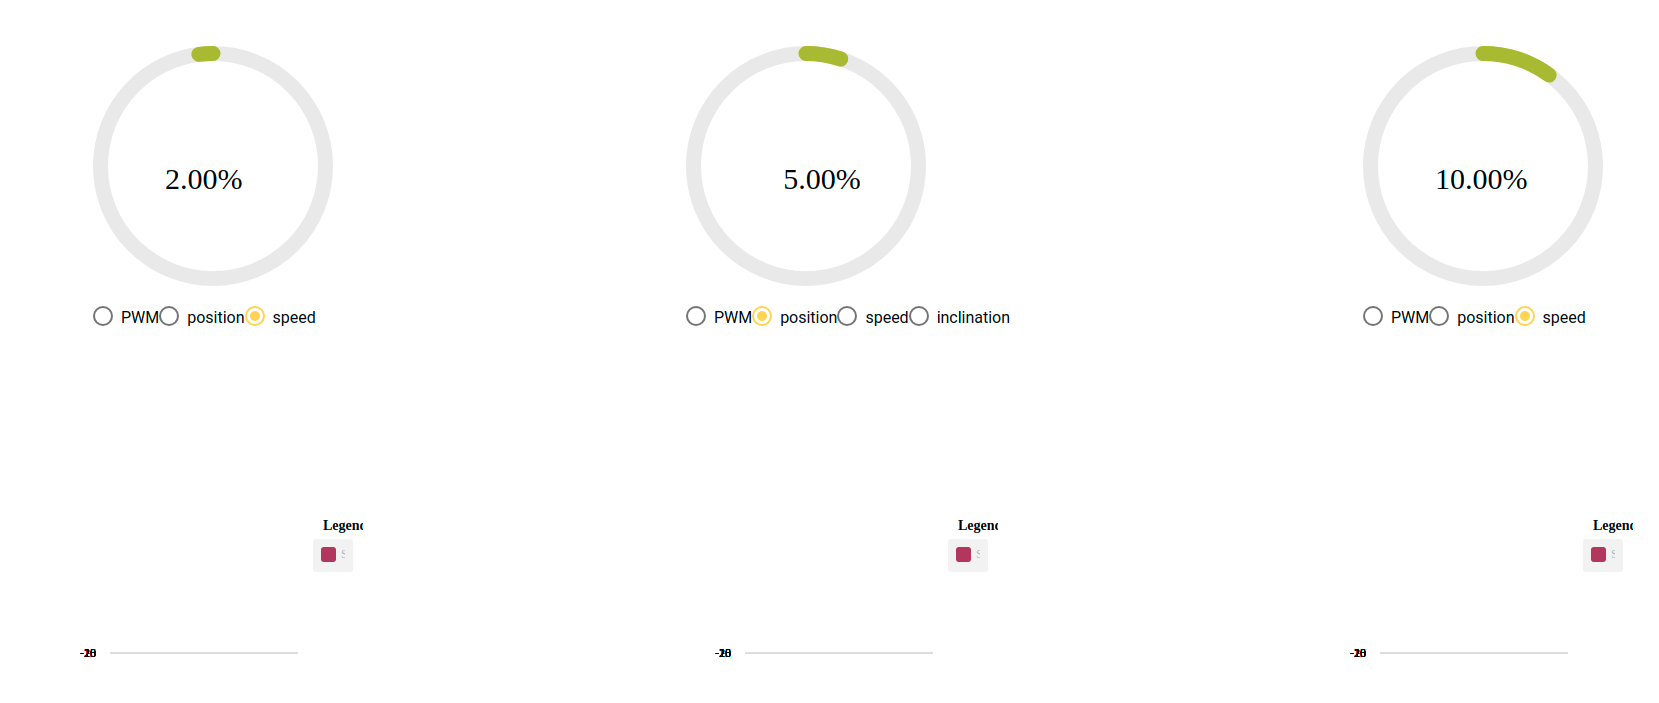
\includegraphics[width=12cm]{img/components/ui.png}
    \caption{Screen shoot of the UI.}
    \label{fig: UI}
\end{figure}
The user interface can be controlled by the keyboard or by a joy-stick connected to the computer. In our case
we used a PS4 remote controller connected via bluetooth to the computer.

The interface whole interface was programed with Angular, a TypeScript framework designed to code user interfaces.
It is organaized in modulus and packages that one can install, as the round progress bar. An Angular Server is 
running in the client machine that can connect to the interface via website.

\subsection{Planner}
The planner main job is to receive and sent sockets to the UI and the controller. Sockets is a method to communicate
different process across the internet with very low latency. The planner is working on a server with a public IP
so the other computers know where they have to exchange the information even if the UI or the Controller changes its IP.

\subsection{Controller}
The controller is running on the Raspberry Pi. The controller has a main file (controller.js) that reads
a configuration file (config.json) and creates instances of the components described on the configuration file.
Once all components are created, it starts different threads for each of the components.

The different components we have are: accelerometer, led, motor and stabilizer. Also we have two auxiliary classes that are
not components: PID and average filter. All the components that rely on hardware are using C++ code to optimize
the code. This code is wrapped in TypeScript classes to make an easier integration of sockets and JSON files.
